\chapter{Code dans la carte principale}

\section{Introduction}
Ce chapitre a pour but de présenter l'architecture logicielle développée lors du précédent projet de Bachelor par Thomas Freyche. Plusieurs illustrations sont d'ailleurs issues de son rapport \cite{Freyche}. Une optimisation de ce code source sera également proposée et détaillée.

\section{Information notable}
Afin d'optimiser l'appropriation du code source hérité, une première révision syntaxique a été réalisée à l'aide d'outils d'intelligence artificielle. Cette démarche avait pour objectif d'améliorer la structure du programme, d'enrichir les commentaires et d'en accroître la lisibilité globale. Le comportement de la maquette a été rigoureusement contrôlé à la suite de cette restructuration purement formelle. Les résultats obtenus étant strictement identiques à ceux de la version d'origine, il est confirmé que cette intervention n'a introduit aucun dysfonctionnement supplémentaire.

\section{Mise en place de CCS}
\label{sec:MiseEnPlace}
\subsection{Installation de Code Composer Studio}
Afin de programmer correctement le DSP, une version spécifique de Code Composer Studio (CCS) ainsi qu'une bibliothèque dédiée au DSP doivent être installées.

La version requise de CCS est la suivante \cite{CCS_Install} :
\url{https://www.ti.com/tool/download/CCSTUDIO/12.6.0} \\

Pour la bibliothèque C2000Ware, la version suivante doit être installée \cite{C2000_Install} :
\url{https://www.ti.com/tool/download/C2000WARE/5.02.00.00}\\

\subsection{Configuration de CCS}

Une fois l'installation terminée, il est nécessaire de configurer CCS pour qu'il détecte la bibliothèque. La procédure d'intégration est la suivante :

\begin{enumerate}
    \item Lancer Code Composer Studio.

    \item Accéder au menu \textit{Window > Preferences}.

    \item Dans la colonne de gauche, naviguer vers \textit{Code Composer Studio > Products}.

    \item Vérifier la liste "Product discovery path". Si le dossier \verb|C:\ti| n'y figure pas, cliquer sur \textit{Add...} et le sélectionner.
    \item Cliquer sur le bouton \textit{Refresh}.

    \item La bibliothèque C2000Ware doit apparaître dans la liste « Discovered products ». Cliquer alors sur \textit{Install}.

    \item Si l'explorateur de fichiers s'ouvre, sélectionner l'emplacement exact du dossier (généralement \verb|C:\ti\c2000\C2000Ware_5_02_00_00|).

    \item Vérifier que le dossier est correctement coché et cliquer sur \textit{Apply and close}. La figure \ref{fig:Res_conf_C2000} illustre le résultat attendu.

          \begin{figure}[H]
              \centering
              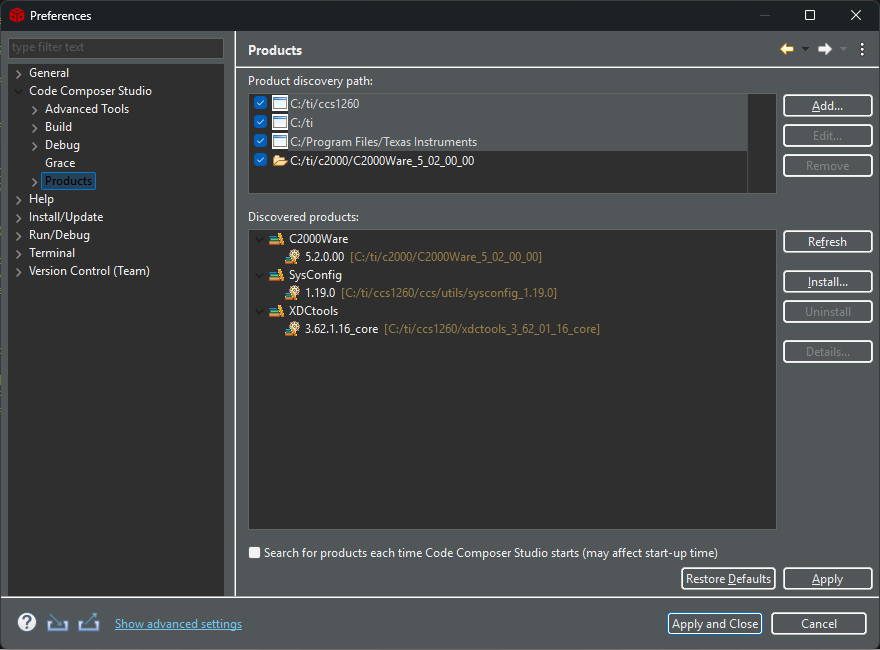
\includegraphics[width=0.75\linewidth]{Image/Chap.2/Resultat_conf_C2000.png}
              \caption{Résultat de la configuration du C2000}
              \label{fig:Res_conf_C2000}
          \end{figure}

    \item Une fois la configuration terminée, cliquer sur le bouton \textit{Build} pour appliquer les changements.
\end{enumerate}

Enfin, il est impératif de vérifier que le niveau d'optimisation de CCS est correctement établi en suivant ces étapes :

\begin{enumerate}
    \item Effectuer un clic droit sur le projet.

    \item Sélectionner \textit{Properties}.

    \item Dérouler l'onglet \textit{Build > C2000 Compiler > Optimization}.

    \item Appliquer les paramètres tels qu'illustrés dans la fenêtre suivante :

          \begin{figure}[H]
              \centering
              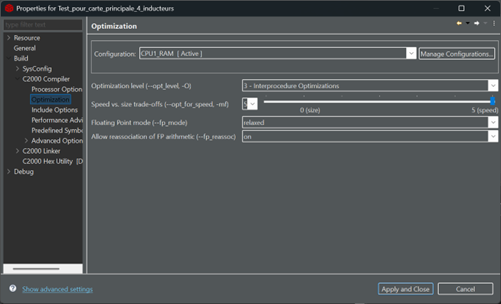
\includegraphics[width=0.75\linewidth]{Image/Chap.2/CCS_Opti_Windows.png}
              \caption{Configuration des paramètres d'optimisation}
              \label{fig:Res_conf_Opti}
          \end{figure}
\end{enumerate}

Lorsque le programme final est prêt, il faudra à ce moment-là flasher le code dans la mémoire flash afin que le code reste en "stand alone".

Il est désormais possible d'utiliser CCS pour la programmation du DSP.

\section{Code de départ}
Cette section traite du fichier principal (\texttt{hrpwm\_ex1\_duty\_sfo.c}) développé pour assurer la sustentation du démonstrateur. Son programme étant dense, son entièreté ne sera pas présentée. Seules les portions de code considérées comme structurantes seront détaillées.

Ce fichier centralise l'ensemble de la logique de commande, particulièrement la régulation, l'acquisition des données ADC et la communication sans fil. Les fonctionnalités implémentées sont les suivantes :

\begin{itemize}
    \item Gestion des interruptions.
    \item Lecture de 8 canaux ADC (mesures de position et de courant par inducteur).
    \item Conversion des valeurs brutes de l'ADC en grandeurs physiques.
    \item Procédure de lancement de la sustentation.
    \item Régulation de position par retour d'état.
    \item Régulation de courant par le biais de régulateurs PI.
    \item Calcul des rapports cycliques (PWM) générés par les boucles de régulation.
    \item Affectation des signaux PWM aux broches de commande des ponts en H.
    \item Communication UART avec le module ESP32.
\end{itemize}

\subsection{Algorithme du code principal}
Actuellement, l'algorithme du programme principal respecte l'organigramme suivant :

\begin{figure}[H]
    \centering
    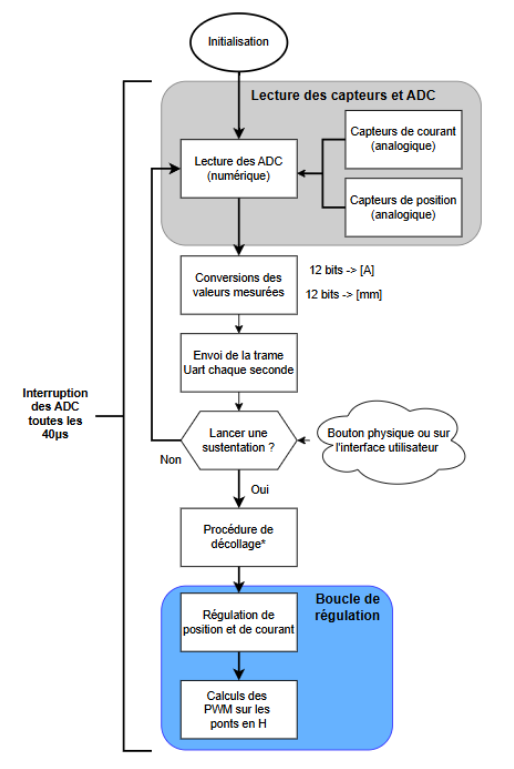
\includegraphics[width=0.7\linewidth]{Image/Chap.2/Algorithme.png}
    \caption{Structure de l'algorithme du code principal \cite{Freyche}}
    \label{fig:AlgorithmeCodePrincipal}
\end{figure}

La majeure partie du code s'exécute au sein d'une routine d'interruption. Celle-ci englobe l'acquisition et la conversion des valeurs ADC, l'exécution des algorithmes de régulation, la mise à jour des modules PWM ainsi que la gestion de l'interface utilisateur (boutons).

\subsection{Bibliothèques}
Le projet s'appuie sur les dépendances suivantes :

\begin{minted}{c}
#include "driverlib.h"
#include "device.h"
#include "board.h"
#include "sfo_v8.h"
#include "math.h"
#include "stdio.h"
#include "FunctionHeader.h"
\end{minted}

\begin{itemize}
    \item \texttt{driverlib.h} : Bibliothèque fondamentale du DSP TI C2000. Elle met à disposition des fonctions de haut niveau permettant la configuration matérielle (ex. : \texttt{ADC\_readResult}, \texttt{GPIO\_writePin}) en s'affranchissant de la manipulation directe des registres.
    \item \texttt{device.h} : Fichier de configuration spécifique au microcontrôleur utilisé. Il définit les fonctions d'initialisation système requises pour le fonctionnement de l'horloge et des périphériques.
    \item \texttt{board.h} : Fichier généré par l'outil SysConfig (voir section \ref{subsubsec:SysConfig}). Il regroupe les définitions des entrées/sorties paramétrées via l'interface graphique.
    \item \texttt{sfo\_v8.h} : Bibliothèque indispensable pour l'exploitation de la fonctionnalité HRPWM (High-Resolution PWM). Elle assure une calibration continue des signaux afin de compenser les dérives thermiques et les fluctuations de tension.
    \item \texttt{math.h} et \texttt{stdio.h} : Bibliothèques standards C dédiées aux calculs mathématiques et à la gestion des flux d'entrées/sorties.
    \item \texttt{FunctionHeader.h} : Fichier d'en-tête local regroupant les définitions paramétriques spécifiques à la maquette (détaillé dans la section \ref{subsubsec:FunctionHeader}).
\end{itemize}

\subsubsection{SysConfig}
\label{subsubsec:SysConfig}
L'outil SysConfig, exploité au travers du fichier \texttt{hrpwm\_ex1\_duty\_sfo.syscfg}, offre une interface de configuration graphique du DSP. Son utilisation permet d'initialiser les modules suivants :

\begin{itemize}
    \item Les convertisseurs analogiques-numériques (ADC).
    \item Les générateurs de signaux PWM.
    \item Le module de communication série SCI (UART).
\end{itemize}

L'interface propose une vue schématique du microcontrôleur simplifiant l'affectation des broches (pin mapping). Lors de la validation de cette configuration, l'outil génère automatiquement les fichiers sources \texttt{board.h} et \texttt{board.c}.

\subsubsection{\texttt{FunctionHeader2.h} et \texttt{FunctionHeader2.c}}
\label{subsubsec:FunctionHeader}
Ces fichiers regroupent l'ensemble des définitions de constantes et des prototypes de fonctions exploités dans le projet. Les éléments qui y sont définis incluent :

\begin{itemize}
    \item Les paramètres physiques : caractéristiques mécaniques et électromagnétiques de la maquette (entrefer nominal, masse, inductance et géométrie des bobines).
    \item Les configurations électriques : tension du bus continu (48~V) et résolution de quantification de l'ADC (12~bits).
    \item Les paramètres PWM : fréquence de découpage (25~kHz), gestion des temps morts (dead bands) des MOSFET et corrections temporelles associées.
    \item Les paramètres de la régulation de courant (PI) : seuil de courant au décollage (3~A), ainsi que les gains de régulation $K_p$, $\tau_i$ et $G_i$.
    \item Les paramètres de la régulation de position (Espace d'état) : coefficients de rétroaction $K_\omega$, $K_d$ et $K_r$.
    \item Les filtres numériques : dimensionnement des fenêtres et coefficients propres aux filtres IIR, FIR et de Savitzky-Golay.
\end{itemize}

Ces fichiers constituent une révision du travail initial mené par Thomas Freyche. Afin d'améliorer la clarté et la modularité du code source, les définitions ont été scindées sur deux fichiers distincts, bien que la logique de fonctionnement demeure strictement identique.

\subsection{Fonctions principales}

\subsubsection{La fonction \texttt{PI\_current\_regulator}}
L'implémentation de la fonction \texttt{PI\_current\_regulator} se présente ainsi :

\begin{minted}{c}
void PI_current_regulator(float ic, float current, float *integral,
float *ue, float *uc){
    float ie = (ic - current) * KP_I;
    *integral += (ie - *ue) * GI_I * H;
    float uc_prim = ie + *integral;

    *uc = uc_prim;
    if (uc_prim > UMAX) {
        *uc = UMAX;
    }
    if (uc_prim < 0) {
        *uc = 0;
    }

    *ue = (uc_prim - *uc) * ANTIWINDUP_EN;
}
\end{minted}

Cette fonction assure la régulation du courant au moyen d'une structure PI. Les arguments qui lui sont passés sont :

\begin{itemize}
    \item Le courant de consigne \texttt{ic}.
    \item Le courant réel mesuré \texttt{current}.
    \item Le pointeur de la variable d'intégration \texttt{integral}.
    \item Le pointeur de l'erreur de tension \texttt{ue}.
    \item Le pointeur de la tension de commande calculée \texttt{uc}.
\end{itemize}

La séquence de régulation s'articule selon les étapes suivantes :

\begin{enumerate}
    \item Calcul de l'erreur $i_e$ (différence entre la consigne et la mesure du courant), puis multiplication par le gain proportionnel.
    \item Mise à jour de l'action intégrale par sommation de la différence entre l'erreur de courant $i_e$ et l'erreur de tension $u_e$, pondérée par le gain intégral $GI_I$ et la période d'échantillonnage $H$.
    \item Évaluation de la commande intermédiaire $u_{c\_prim}$, obtenue par la somme des actions proportionnelle et intégrale.
    \item Saturation de la commande afin de respecter les limites physiques imposées par l'alimentation de la maquette (plage de 0~V à $U_{MAX}$ = 48~V). La consigne finale est restreinte à ces bornes le cas échéant.
    \item Calcul de l'écart de tension (différence entre la commande intermédiaire et la commande saturée) pondéré par le coefficient d'anti-windup, afin de prévenir l'emballement de l'intégrateur.
\end{enumerate}

Cette fonction est appelée de manière cyclique dans la routine d'interruption principale pour assurer l'asservissement en courant des quatre bobines.

\subsubsection{Filtre de Savitzky}
\label{subsubsec:Savitzky}
Le code du filtre de Savitzky-Golay est implémenté de la façon suivante :

\begin{minted}{c}
float savitzky_Filter(float *Buffer)
{
    float v = 0.0f;
    uint16_t m = 0;

    for(m = 0; m < FILTWINDOW; m++)
        v += F_PWM*Buffer[m]*SAVITZKY[m];

    for(m = 0; m < FILTWINDOW-1; m++)
        Buffer[m] = Buffer[(m+1)];

    return v;
}
\end{minted}

Ce filtre \cite{Savitzky} est utilisé pour lisser les mesures fortement bruitées tout en conservant fidèlement la dynamique temporelle du signal utile.

Le principe de fonctionnement est illustré par la figure \ref{fig:PrincipeSavitzky} :

\begin{figure}[H]
    \centering
    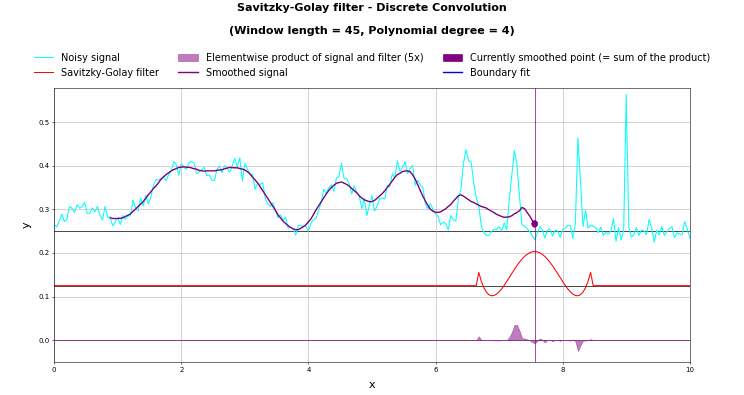
\includegraphics[width=1\linewidth]{Image/Chap.2/PrincipeSyvitzky.png}
    \caption{Principe de lissage du filtre de Savitzky-Golay \cite{Savitzky}}
    \label{fig:PrincipeSavitzky}
\end{figure}

Le traitement s'apparente à l'application d'un filtre FIR à fenêtre glissante. Dans son paramétrage actuel, la fonction mémorise les neuf dernières acquisitions de position. Une somme pondérée est calculée en multipliant chaque échantillon par un coefficient propre au filtre de Savitzky :

\begin{minted}{c}
//savitzky filter coefficients, order = 2, window = 9
const float SAVITZKY[FILTWINDOW] = {-0.0667, -0.05, -0.0333, -0.0167,
                                     0.0, 0.0167, 0.0333, 0.05, 0.0667};
\end{minted}

Un élargissement de la fenêtre de glissement permet de renforcer l'atténuation du bruit, mais ce lissage s'obtient au détriment du temps d'exécution (charge processeur). Ce filtre est spécifiquement exploité dans le firmware pour atténuer le bruit d'acquisition des canaux ADC dédiés aux capteurs de position (voir section \ref{subsubsec:ADC}).

\subsubsection{Filtre IIR}
L'algorithme du filtre IIR (Infinite Impulse Response) est rédigé comme suit :

\begin{minted}{c}
float IIR_Filter(float *entree, float *sortie)
{
    float somme = 0.0;
    float somme2 = 0.0;

    uint16_t k = 0;

    //difference equation
    for(k = 0; k < Nb; k++) //Num.
        somme += b[k]*entree[k];
    for(k = 0; k < Na; k++) //Den.
        somme2 += a[k]*sortie[k];

    //update buffers
    for(k = (Na-1); k > 0; k--)
        sortie[k] = sortie[(k-1)];

    sortie[0] = (somme-somme2);

    for(k = (Nb-1); k > 0; k--)
        entree[k] = entree[(k-1)];

    return (somme-somme2);
}
\end{minted}

La topologie retenue pour ce filtre correspond à un réjecteur de bande (filtre coupe-bande). Son rôle consiste à atténuer une perturbation de résonance observée autour de 75~Hz. Si l'origine physique précise de cette oscillation reste à ce jour inexpliquée, son atténuation est une condition stricte pour maintenir la stabilité des boucles de régulation.\\

Les coefficients paramétrés sont les suivants :

\begin{minted}{c}
    //bandstop Filter 75Hz 2nd order bande coupe de 40Hz  130Hz (6)
#define A1_B1_6         -1.977307757140243538
#define A2_6            0.97763254912161579
#define B0_B2_6         0.98881627456080789517756
\end{minted}

Toutefois, lors de l'analyse du code source hérité, il a été constaté que ces définitions n'étaient pas utilisées. Une autre variante de coefficients était active :

\begin{minted}{c}
//bandstop Filter 56Hz 2nd order bande coupe de 47Hz  90Hz (0) (test)
#define A1_B1_0         -1.980143772501098
#define A2_0            0.980339665209542
#define B0_B2_0         0.9901698326047711
\end{minted}

Cette disparité provient vraisemblablement d'essais expérimentaux antérieurs non documentés. Par souci de cohérence avec le travail de Laucella \cite{Laucella}, les paramètres ciblant la fréquence de 75~Hz ont été restaurés.

\section{Mesure du temps de l'interruption principale}
L'une des premières hypothèses formulées a été que le code ne respectait pas le temps d'exécution alloué pour l'interruption complète. Il a donc été nécessaire de vérifier la validité des temps de cycle, de mesurer le temps consommé par chaque sous-routine, et de déterminer si l'interruption liée à la communication entre le DSP et l'ESP32 perturbait l'interruption principale.\\

Le protocole de mesure a consisté à évaluer le système avec les quatre inducteurs actifs, puis uniquement avec l'avant (inducteurs 1 et 2), et enfin uniquement avec l'arrière (inducteurs 3 et 4). Ces mesures ont été réalisées avec et sans l'activation de l'interruption de la liaison UART afin d'établir une comparaison. Pour rappel, la période de l'interruption principale est de 40~$\mu$s.

L'analyse temporelle se concentre sur quatre phases de l'interruption : premièrement, l'interruption dans son entièreté ; deuxièmement, le temps consommé par les conversions ADC ; troisièmement, le temps d'exécution de la machine d'états ; et enfin, le temps dédié à la mise à jour des signaux PWM. Les relevés ont été effectués à l'aide d'un oscilloscope en observant les commutations d'une broche de sortie (LED).\\

\subsection{Relevé des mesures}
Les mesures sont recensées dans le tableau \ref{tab:verif_temps_final} :

\begin{table}[H]
    \centering
    \resizebox{\textwidth}{!}{%
        \begin{tabular}{|l|c|c|c|c|c|c|}
            \hline
            \multicolumn{7}{|c|}{\textbf{Vérification des temps}}                                                                                                                                                                                                                                                                                                                                                                                                                                                  \\ \hline
            \multicolumn{1}{|c|}{\multirow{2}{*}{\textbf{Mesure}}} & \multicolumn{3}{c|}{\textbf{Avec UART}}                             & \multicolumn{3}{c|}{\textbf{Sans UART}}                                                                                                                                                                                                                                                                                                                                 \\ \cline{2-7}
            \multicolumn{1}{|c|}{}                                 & \begin{tabular}[c]{@{}c@{}}4 Inducteurs\\ {[}$\mu$s{]}\end{tabular} & \begin{tabular}[c]{@{}c@{}}Inducteurs\\ 1\&2 {[}$\mu$s{]}\end{tabular} & \begin{tabular}[c]{@{}c@{}}Inducteurs\\ 3\&4 {[}$\mu$s{]}\end{tabular} & \begin{tabular}[c]{@{}c@{}}4 Inducteurs\\ {[}$\mu$s{]}\end{tabular} & \begin{tabular}[c]{@{}c@{}}Inducteurs\\ 1\&2 {[}$\mu$s{]}\end{tabular} & \begin{tabular}[c]{@{}c@{}}Inducteurs\\ 3\&4 {[}$\mu$s{]}\end{tabular} \\ \hline
            Interruption globale                                   & 20                                                                  & 13.6                                                                   & 14.4                                                                   & 20.4                                                                & 14                                                                     & 14.4                                                                   \\ \hline
            ADC                                                    & 0.88                                                                & 0.86                                                                   & 0.84                                                                   & 0.88                                                                & 0.86                                                                   & 0.85                                                                   \\ \hline
            Machine d'état                                         & 13.2                                                                & 9.4                                                                    & 9.4                                                                    & 13.6                                                                & 9.6                                                                    & 9.6                                                                    \\ \hline
            PWM                                                    & 5.2                                                                 & 2.6                                                                    & 2.92                                                                   & 4.9                                                                 & 2.76                                                                   & 2.96                                                                   \\ \hline
        \end{tabular}%
    }
    \caption{Vérification des temps d'exécution avec et sans UART}
    \label{tab:verif_temps_final}
\end{table}

Les chronogrammes détaillés des mesures temporelles sont disponibles dans l'annexe \ref{an:MesTemps}.

\subsection{Analyse des résultats}
Comme l'illustre le tableau \ref{tab:verif_temps_final}, aucun temps d'exécution ne dépasse la période allouée à l'interruption. Une marge temporelle importante reste disponible. L'origine du dysfonctionnement global n'est donc pas liée à une surcharge du processeur, ce qui confirme la viabilité de l'interruption principale et de l'interruption de communication. Celles-ci n'entrent pas en conflit et s'exécutent sans se bloquer mutuellement.

\section{Réalisation d'une nouvelle machine d'états}
La machine d'états précédente présentant une architecture complexe et difficilement lisible, il a été décidé de la restructurer intégralement. Le comportement séquentiel défini est le suivant :

\begin{itemize}
    \item État 0 : Attente de la pression du bouton d'activation.
    \item État 1 : Montée du courant des inducteurs 1 et 2 à 3~A (afin d'éviter un démarrage à zéro).
    \item État 2 : Augmentation du courant des inducteurs 1 et 2 suivant une rampe continue (régulation de courant seule).
    \item État 3 : Basculement en régulation de position dès l'amorce du mouvement des inducteurs 1 et 2 (lévitation de la partie avant du véhicule).
    \item État 4 : Montée du courant des inducteurs 3 et 4 à 3~A.
    \item État 5 : Augmentation du courant des inducteurs 3 et 4 suivant une rampe continue (régulation de courant seule).
    \item État 6 : Basculement en régulation de position dès l'amorce du mouvement des inducteurs 3 et 4 (lévitation de la partie arrière, l'avant étant déjà sustenté).
    \item État 7 : Ajustement des gains statiques pour assurer un comportement transitoire plus doux et passage en régulation de maintien.
    \item État 8 : Arrêt de la sustentation et réinitialisation des variables.
    \item État 9 : Affichage d'un message d'erreur en cas de défaillance matérielle ou logicielle de la maquette.
\end{itemize}

Conformément à ces spécifications, l'organigramme de la figure \ref{fig:MachineDEtat} a été établi :

\begin{figure}[H]
    \centering
    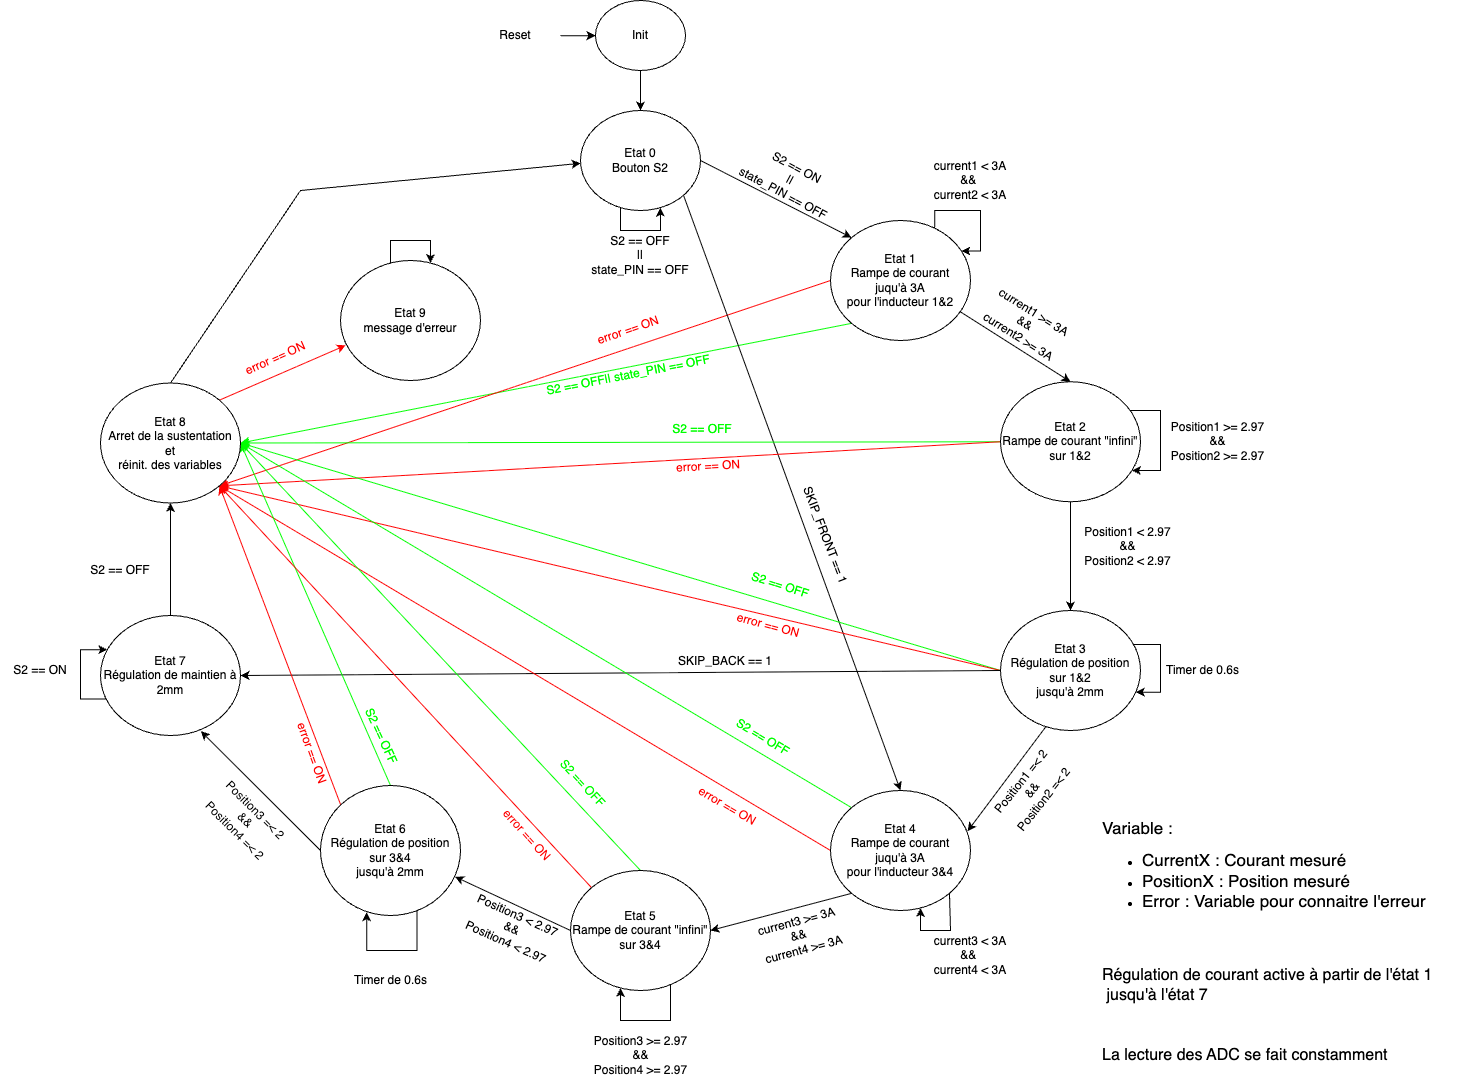
\includegraphics[width=1\linewidth]{assets/Chap5/MachineDEtat.png}
    \caption{Machine d'états régissant la séquence de lévitation}
    \label{fig:MachineDEtat}
\end{figure}

Le diagramme détaillé de cette machine d'états est également disponible dans l'annexe \ref{an:MachineDetat}.\\

Les différents états sont implémentés dans le code source en respectant scrupuleusement la logique illustrée par la figure \ref{fig:MachineDEtat}.\\

Les états 0 et 8 sont actuellement structurés par de simples conditions logiques :

\begin{minted}{c}
    // State 0 :
    // Vérification de l'enclenchement de la régulation
    if(ButtonS2 || state_PIN)
    {
        ...
    }
    // State 8 :
    // Arrêt de la sustentation
    else if(!ButtonS2 || !state_PIN)
    {
        ...
    }
\end{minted}

L'état 1 est programmé de la manière suivante :

\begin{minted}{c}
    // State 1 :
    // Rampe de courant sur les inducteur 1&2 jusqu'à atteindre les 3A
    case STATE_1:

        // Rampe vers 3A par pas de 0.04A
        if(ic1 < I_SP)
        {
            ic1 += TAKEOFF_CURRENT_STEP1;
        }
        else
        {
            ic1 = I_SP;
        }

        // Fixe le courant de consigne 2 par rapport à ic1
        ic2 = ic1;

        mean1 += Current1;
        mean2 += Current2;
        dt_mean++;

        if(dt_mean >= 200) // dt = 8ms
        {
            mean1 = mean1 / dt_mean;
            mean2 = mean2 / dt_mean;

            if((mean1 <= I_SP105 && mean1 >= I_SP095) && (mean2 <= I_SP105 && mean2 >= I_SP095))
            {
                // Reset des variables
                mean1 = 0;
                mean2 = 0;
                dt_mean = 0;

                // Changement d'état
                state = STATE_2;

            }
            else
            {
                // Reset des variables pour mesurer à nouveau
                mean1 = 0;
                mean2 = 0;
                dt_mean = 0;
            }
        }

        break;
\end{minted}

L'état 2 s'exécute selon la logique suivante :

\begin{minted}{c}
    // State 2 :
    // Rampe de courant "infinie" pour atteindre un courant
    // assez grand pour faire décoller l'avant
    case STATE_2:

        if(Position1 <= Position_c1_dec && Position2 <= Position_c2_dec)
        {
            // Update des variables
            Position_c1 = Position1;
            Position_c2 = Position2;

            // Changement d'état
            state = STATE_3;
        }
        else if(ic1 < 7.82f)
        {
            ic1 += TAKEOFF_CURRENT_STEP1;
        }
        else
        {
            // Fixe le courant à une valeur max
            ic1 = 7.82f;
        }

        // Fixe le courant de ic2 à ic1
        ic2 = ic1;

        break;
\end{minted}

L'état 3 est défini par le bloc de code ci-dessous :

\begin{minted}{c}
    // State 3 :
    // Activation de la régulation de position pour atteindre les 2mm
    // à l'avant
    case STATE_3:

        // Activer la régulation d'état
        if(!PosRegFlag1) PosRegFlag1 = true;

        // Set point generator (Ramp from 3mm to 2mm)
        if(Position_c1 > DELTA_N)
        {
            Position_c1 -= 2.5 * 4e-7;
        }
        else
        {
            Position_c1 = DELTA_N;
        }

        if(Position_c2 > DELTA_N)
        {
            Position_c2 -= 2.5 * 4e-7;
        }
        else
        {
            Position_c2 = DELTA_N;
        }

        // Incrémentation du timer
        i_store++;

        // Timer pour attendre un peu pour être sur que le système à bien décoller
        if(i_store == I_STORE_2E_DECOLLAGE)
        {
            // Reset de la varibale
            i_store = 0;

            if(SKIP_BACK)
            {
                state = STATE_7;
            }
            else
            {
                state = STATE_4;
            }
        }

        break;
\end{minted}

L'état 4 repose sur la structure suivante :

\begin{minted}{c}
    // State 4 :
    // Rampe de courant sur les inducteur 3&4 jusqu'à atteindre les 3A
    case STATE_4:

        // Rampe vers 3A par pas de 0.04A
        if(ic3 < I_SP)
        {
            ic3 += TAKEOFF_CURRENT_STEP1;
        }
        else
        {
            ic3 = I_SP;
        }

        // Fixe le courant de consigne 4 par rapport à ic3
        ic4 = ic3;

        mean3 += Current3;
        mean4 += Current4;
        dt_mean++;

        if(dt_mean >= 200) // dt = 8ms
        {
            mean3 = mean3 / dt_mean;
            mean4 = mean4 / dt_mean;

            if((mean3 <= I_SP105 && mean3 >= I_SP095) && (mean4 <= I_SP105 && mean4 >= I_SP095))
            {
                // Reset des variables
                mean3 = 0;
                mean4 = 0;
                dt_mean = 0;

                state = STATE_5;
            }
            else
            {
                // Reset des variables pour mesurer à nouveau
                mean3 = 0;
                mean4 = 0;
                dt_mean = 0;
            }
        }

        break;
\end{minted}

L'état 5 est implémenté selon les instructions suivantes :

\begin{minted}{c}
    // State 5 :
    // Rampe de courant "infinie" pour atteindre un courant
    // assez grand pour faire décoller l'arrière
    case STATE_5:

        if(Position3 <= Position_c3_dec && Position4 <= Position_c4_dec)
        {
            // Update des variables
            Position2_c3 = Position3;
            Position2_c4 = Position4;

            // Changement d'état
            state = STATE_6;
        }
        else if(ic3 < 7.82f)
        {
            ic3 += TAKEOFF_CURRENT_STEP1;
        }
        else
        {
            // Fixe le courant à une valeur max
            ic3 = 7.82f;
        }

        // Fixe le courant de ic4 à ic3
        ic4 = ic3;


        break;
\end{minted}

L'état 6 s'articule comme suit :

\begin{minted}{c}
    // State 6 :
    // Activation de la régulation de position pour atteindre les 2mm
    // à l'arrière
    case STATE_6:

        // Activer la régulation d'état
        if(!PosRegFlag3) PosRegFlag3 = true;

        // Set point generator (Ramp from 3mm to 2mm)
        if(Position2_c3 > DELTA_N)
        {
            Position2_c3 -= 2.5 * 4e-7;
        }
        else
        {
            Position2_c3 = DELTA_N;
        }

        if(Position2_c4 > DELTA_N)
        {
            Position2_c4 -= 2.5 * 4e-7;
        }
        else
        {
            Position2_c4 = DELTA_N;
        }

        // Incrémentation du timer
        i_store++;

        // Timer pour attendre un peu pour être sur que le système à bien décoller
        if(i_store == I_STORE_2E_DECOLLAGE)
        {
            // Reset de la varibale
            i_store = 0;

            // Changement du gain statique de l'inducteur 3
            Kr_sans_int = 0; //-1.0;

            // Changement d'état
            state = STATE_7;
        }

        break;
\end{minted}

Enfin, l'état 7 est défini par les instructions de maintien :

\begin{minted}{c}
    // State 7 :
    // Régulation de maintien pour tenir la maquette en l'air
    case STATE_7:

        // Changement des variables pour une régulation plus douce
        Kr = KR_CHANGE;
        Kw = KW_CHANGE;
        Kd = KD_CHANGE;
        Kddot = KDDOT_CHANGE;

        break;

    // Default :
    // Something went wrong so let's just go to state 9 for an error
    default:
        break;
\end{minted}

Actuellement, l'état 9 n'est pas encore développé. À terme, son implémentation sera requise pour assurer la gestion sécurisée des erreurs et défaillances de la maquette.\\

Cette nouvelle machine d'états a été testée et a fourni des résultats nettement plus conformes au comportement espéré. La lévitation s'en trouve stabilisée ; cependant, il reste nécessaire d'optimiser les conditions de transition entre les différents états. Certains critères de basculement apparaissent en effet trop sensibles, à l'image de la détection du décollage basée sur un seuil de 99~\%. Une perturbation ponctuelle ou un bruit de mesure pourrait ainsi être faussement interprété comme un décollage effectif, déclenchant une transition prématurée.\\

Dans l'ensemble, l'architecture de cette nouvelle machine d'états est validée et fonctionnelle.

\section{A faire}
\begin{itemize}
    \item Ajouter un posage de la maquette en doceur
    \item Ajouter la mise à 0 des variables
    \item Améliorer l'état 0 et l'état 8
    \item Rechercher des moyens d'obtenir des messages d'erreurs
\end{itemize}
